\documentclass[11pt]{article}
\usepackage{float}
\usepackage{amsfonts}
\usepackage{amsmath}
\usepackage{multirow}
\usepackage{makecell}
\usepackage{booktabs}
\newcommand\norm[1]{\lVert#1\rVert}
\newcommand\normx[1]{\Vert#1\Vert}
\usepackage[english,ukrainian]{babel}
    \title{\textbf{Применение Recurrent Sigmoid Piecewise нейрона для прогнозирования временных рядов}}
    \date{}
    
    \addtolength{\topmargin}{-3cm}
    \addtolength{\textheight}{3cm}
\usepackage{graphicx}
\begin{document}

\maketitle
\thispagestyle{empty}

\section*{Введение}

Необходимость прогнозировать временные ряды возникает в множестве сфер и контекстов: экономика, социология, метеорология, как составляющая часть различных систем принятия решений и др. На основе прогнозов строятся планы и принимаются решения, а неправильный прогноз может привести к неправильным планам и решениям. Именно поэтому важность и актуальность задачи прогнозирования сложно переоценить. При этом существует множество факторов, значительно усложняющих решение этой задачи: нестационарный характер прогнозируемого объекта/процесса, большой уровень шума в имеющихся данных, малое количество имеющихся данных и другие.
\\
Класические подходы к решению задачи прогнозирования в основном основываются на применении математической статистики и теории вероятности и обычно предполагают как минимум слабую стационарность прогнозируемого объекта или некоторый конкретный вид нестационарности. Использование методов на основе искусственного интеллекта позволяет избавиться от отдельных предположений и недостатков классических подходов. На сегодня наиболее перспективным направлением интеллектуальных технологий считаются искусственные нейронные сети, в том числе благодаря их универсальности и поразительным результатам, полученным в различных сферах их использования, таких как: анализ изображень, видео, текста, языка и другие. Однако, большинство современных методов прогнозирования на основе нейронных сетей и/или других интеллектуальных подходов не решают проблему непостоянного характера прогнозируемого ряда: в случае неожиданного изменения "поведения"\ процесса качество прогноза зачастую значительно ухудшается. Данная работа предлагает схему построения прогнозирующей модели, способной динамически корректировать свои текущие прогнозы исходя из ошибок предыдущих прогнозов.

\section*{Постановка задачи}

Имеется временной ряд ${x_1, ..., x_N}$, сгенерированный некоторым вероятностным процессом $ \{X_t\} $ с неизвестными cовместными распределениями:
$$ p(x_{t+k}, x_{t}, x_{t-1}, ..., x_{t-n}). $$
Процесс $ \{X_t\} $ может быть как стационарным так и нестационарным. Если процесс нестационарный - в общем случае данная задача прогнозирования не имеет решения, так как вероятностные распределения нестационарного ряда в теории могут "меняться"\ как угодно, и распределения в будущем могут не иметь ничего общего с распределениями, на основе которых был сгенерирован имеющийся временной ряд. Однако на практике изменение вероятностных распределений нестационарных процессов с течением времени не происходит совершенно случайным образом. Поэтому прогнозирующие модели, оцененные на имеющемся в наличии временном ряде, обычно работают удовлетворительно на протяжении определенного периода времени даже при условии нестационарности соответствующего процесса.

Необходимо использовать данный временной ряд для нахождения прогнозирующей модели вида:
$$ \hat{x}_{t+k} = f^*(x_{t}, ..., x_{t-n}), $$
которая минимизирует математическое ожидание ошибки:
$$ f^* = argmin_f \{ E_{p(x_{t+k}, x_{t}, x_{t-1}, ..., x_{t-n})} [ L(f(x_{t}, ..., x_{t-n}), x_{t+k}) ] \}, $$
где:
\begin{itemize}
\item $L: \mathbb{R} \times \mathbb{R} \to \mathbb{R}_{\geq 0} $ - функция ошибки, часто используется либо квадратическая $ L(x, \hat{x}) = (x-\hat{x})^2 $ либо абсолютная ошибка $ L(x, \hat{x}) = |x-\hat{x}| $
\item $k$ - горизонт прогнозирования, т.е. на сколько "шагов"\ вперед необходимо выполнить прогноз; данное значение задается исходя из конкретной потребности в прогнозе и является частью постановки задачи
\item $n$ - размер предыстории, т.е. количество предыдущих значений временного ряда, которые используются для получения прогноза.
\end{itemize}
Поскольку рассчитать настоящее математическое ожидание невозможно (соответствующие вероятностные распределения неизвестны), вместо него используется среднее значение функции ошибки на тестовой подвыборке временного ряда:

$$ f^* = argmin_f \{ \frac{1}{M} \sum_{t=N-k-M+1}^{N - k}{L(f(x_t, ..., x_{t-n}), x_{t+k})} \}, $$
где $M$ - количество примеров, входящих в тестовую подвыборку.

\section*{Основные существующие методы прогнозирования}
\textbf{Линейные модели на основе модели ARIMA}.
\\
В основе модели ARIMA лежит более простая модель ARMA, использующаяся для описания временного ряда $X_t$ следующим образом:
$$X_t = c + \sum_{i=1}^{p}{a_iX_{t-i}} + \sum_{j=1}^{q}{b_j\varepsilon_{t-j} + \varepsilon_t},$$
где:
\begin{itemize}
\item $\varepsilon_t$ - стационарный временной ряд, представляющий собой шум с нулевым математическим ожиданием;
\item $ c, a_1, ..., a_p, b_1, ..., b_q $ - параметры модели.
\end{itemize}
Модель ARIMA(p,d,q) обобщает модель ARMA(p, q) используя для этого оператор разности временного ряда порядка $\Delta^d$:
$$\Delta^dX_t = c + \sum_{i=1}^{p}{a_i\Delta^dX_{t-i}} + \sum_{j=1}^{q}{b_j\varepsilon_{t-j} + \varepsilon_t},$$
где $\Delta^d$ - оператор разности временного ряда порядка d (последовательное взятие d раз разностей первого порядка — сначала от временного ряда, затем от полученных разностей первого порядка, затем от второго порядка и т. д.).

Существуют разные методы для построения прогнозирующих ARIMA моделей, среди наиболее известных - линейная регрессия, методология Бокса-Дженкинса, опорная векторная регрессия. Линейная регрессия заключается в построении частного случая ARIMA модели вида:
$$\Delta^dX_t = \sum_{i=1}^{p}{a_i\Delta^dX_{t-i}} + a_0 ,$$
где вектор параметров $\vec{a} = [a_0, a_1, ..., a_p]$ оценивается с помощью метода наименьших квадратов:
$$ \vec{a} = {(A^TA)}^{-1}A^Ty ,$$
где $A, y$ - матрица и вектор получаемые из исходного временного ряда применяя оператор $\Delta^d$ и скользящее окно размера $p$.
\\
Методология Бокса-Дженкинса позволяет оценивать полную ARIMA модель, но часто требует "экспертного вмешательства"\ для определения параметров $p,q,d$, так как существуют различные тесты для их определения, и необходимо выбирать тот либо иной тест и критические значения выбранного теста.
\\
Метод опорной векторной регрессии применяет идеи метода опорных векторов к задаче регрессии: для заданных пар $x_i, y_i; x_i \in \mathbb{R}^n, y_i \in \mathbb{R}, i=1,...,N$ (полученных после применения скользящего окна к исходному временному ряду) оптимальная линейная модель $\hat{y_i} = f(x_i;w) = \sum_{i=1}^{n}{w_ix_i} + w_0$ находится путем решения оптимизационной задачи:
$$ minimize: \frac{1}{2}\norm{w}^2 $$
$$ where: |y_i - f(x_i;w)| \le \varepsilon, i=1,...,N, $$
где $ \varepsilon \ge 0 $ - порог допустимой ошибки модели. В случае наличия случайных выбросов в обучающих данных вводятся дополнительные переменные $ \xi_i, \xi^*_i $ и регуляризационный параметр $ C > 0 $ (выбираемый "вручную") и решается новая задача:
$$ minimize: \frac{1}{2}\norm{w}^2 + C\sum_{i=1}^{N}{(\xi_i + \xi^*_i)} $$
$$ where: $$
$$ y_i - f(x_i; w) \le \varepsilon + \xi^*_i, i=1,...,N $$
$$ f(x_i; w) - y_i \le \varepsilon + \xi_i, i=1,...,N $$
$$ \xi_i, \xi^*_i \ge 0, i=1,...,N. $$
Также существуют нелинейные варианты метода опорной регрессии на основе применения функций-ядер. 
\\
\textbf{Искусственные нейронные сети}.
\\
Искусственные нейронные сети представляют собой систему взаимосвязанных искусственных нейронов, где каждый нейрон обычно реализует простую функцию вида:
$$ f(x;w) = u(w \cdot x); x,w \in \mathbb{R}^n $$
где $u: \mathbb{R} \to \mathbb{R} $ - некоторая нелинейная функция, называемая функцией активации; $ w $ - вектор весовых коэффициентов нейрона, настраиваемых в процессе обучения сети. Наиболее популярные функции активации:
\begin{itemize}
\item $ReLU(x;w) = max(0,w \cdot x)$
\item $ \sigma(x;w) = \frac{1}{1 + e^{-w \cdot x}} $
\item $ tanh(x;w) = tanh(w \cdot x) = \frac{2}{1 + e^{-2 w \cdot x}} - 1$
\end{itemize}
В контексте задачи прогнозирования популярными являются искусственные нейронные сети прямого распространения (feedforward neural network) со структурой вида:
\begin{figure}[H]
\centering
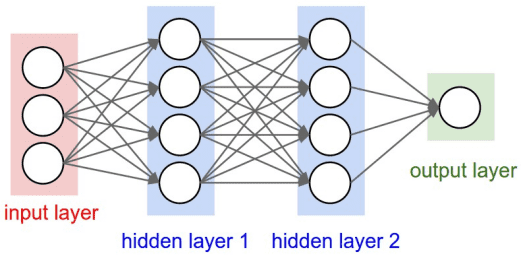
\includegraphics[scale=0.4]{ff-neural-net.png}
\label{}
\end{figure}
которые по сути являются нелинейной вариацией AR-модели: $X_t = f(X_{t-1},...,X_{t-p})$ - где $f$ - функция, реализуемая нейронной сетью.
Настройка параметров нейронной сети, также называемая обучением, обычно производится применением некоторой вариации алгоритма градиентного спуска:
\begin{itemize}
\item Для относительно небольших сетей и временных рядов можно применять алгоритм Левенберга-Марквардта, который на практике часто находит значение параметров, близкое к оптимальному, и делает это значительно быстрее других алгоритмов (опять же, при условии небольшого количества параметров и длины временного ряда). 
\item Для больших сетей но относительно коротких временных рядов часто применяют "стандартный"\ алгоритм градиентного спуска либо его модификации типа алгоритма Adam, LBFGS, где градиент рассчитывается сразу для всего временного ряда.
\item Для больших сетей и длинных временных рядов используются "пакетные"\ вариации алгоритмов из предыдущего пункта, в которых на каждой итерации градиент рассчитывается только для определенного под-множества - "пакета"\ данных.
\end{itemize}
Кроме оптимизации непосредственно параметров нейронной сети с заданной структурой также необходимо определить саму структуру сети. Кроме варианта применения определенных эвристик для "ручного"\ задания структуры также возможно применение алгоритмов автоматического подбора структуры: наиболее популярными являются алгоритмы обучения с подкреплением, эволюционные алгоритмы и алгоритмы семейства МГУА. Основные алгоритмы семейства МГУА были созданы до того, как искусственные нейронные сети стали популярными, поэтому их часто рассматривают как отдельные методы. Однако их также можно рассматривать как различные способы оптимизации структуры и параметров полиномиальных нейронных сетей, в которых используются нейроны с функциональной моделью в виде полиномов Колмогорова-Габора:
$$ f(x;w) = w_0 + \sum_{i=1}^{n}{w_ix_i} + \sum_{i=1}^{n}{\sum_{j=i}^{n}{w_{ij}x_ix_j}} + \sum_{i=1}^{n}{\sum_{j=i}^{n}{\sum_{k=j}^{n}{w_{ijk}x_ix_jx_k}}} + ... $$
\\
\textbf{Рекуррентные нейронные сети}.
\\
В задачах обработки ествественного языка, таких как построение языковых моделей, автоматический перевод текста и пр. хорошо себя "зарекомендовали" рекуррентные нейронные сети на основе Long Short Term Memory (LSTM) и/или Gated Recurrent Unit (GRU) нейронов. Данные нейроны имеют схожую структуру, которая позволяет уменьшить влияние проблемы затухающего/взрывающегося градиента при обучении рекуррентных моделей с использованием Backpropagation Through time (BPTT) алгоритма на длинных последовательностях. За счет этого, на практике, сети с этими нейронами более стабильны в обучении и имеют большую "точность" при работе на длинных последовательностях. LSTM-нейрон имеет следующую структуру:
\\
\\
\begin{figure}[h]
\centering
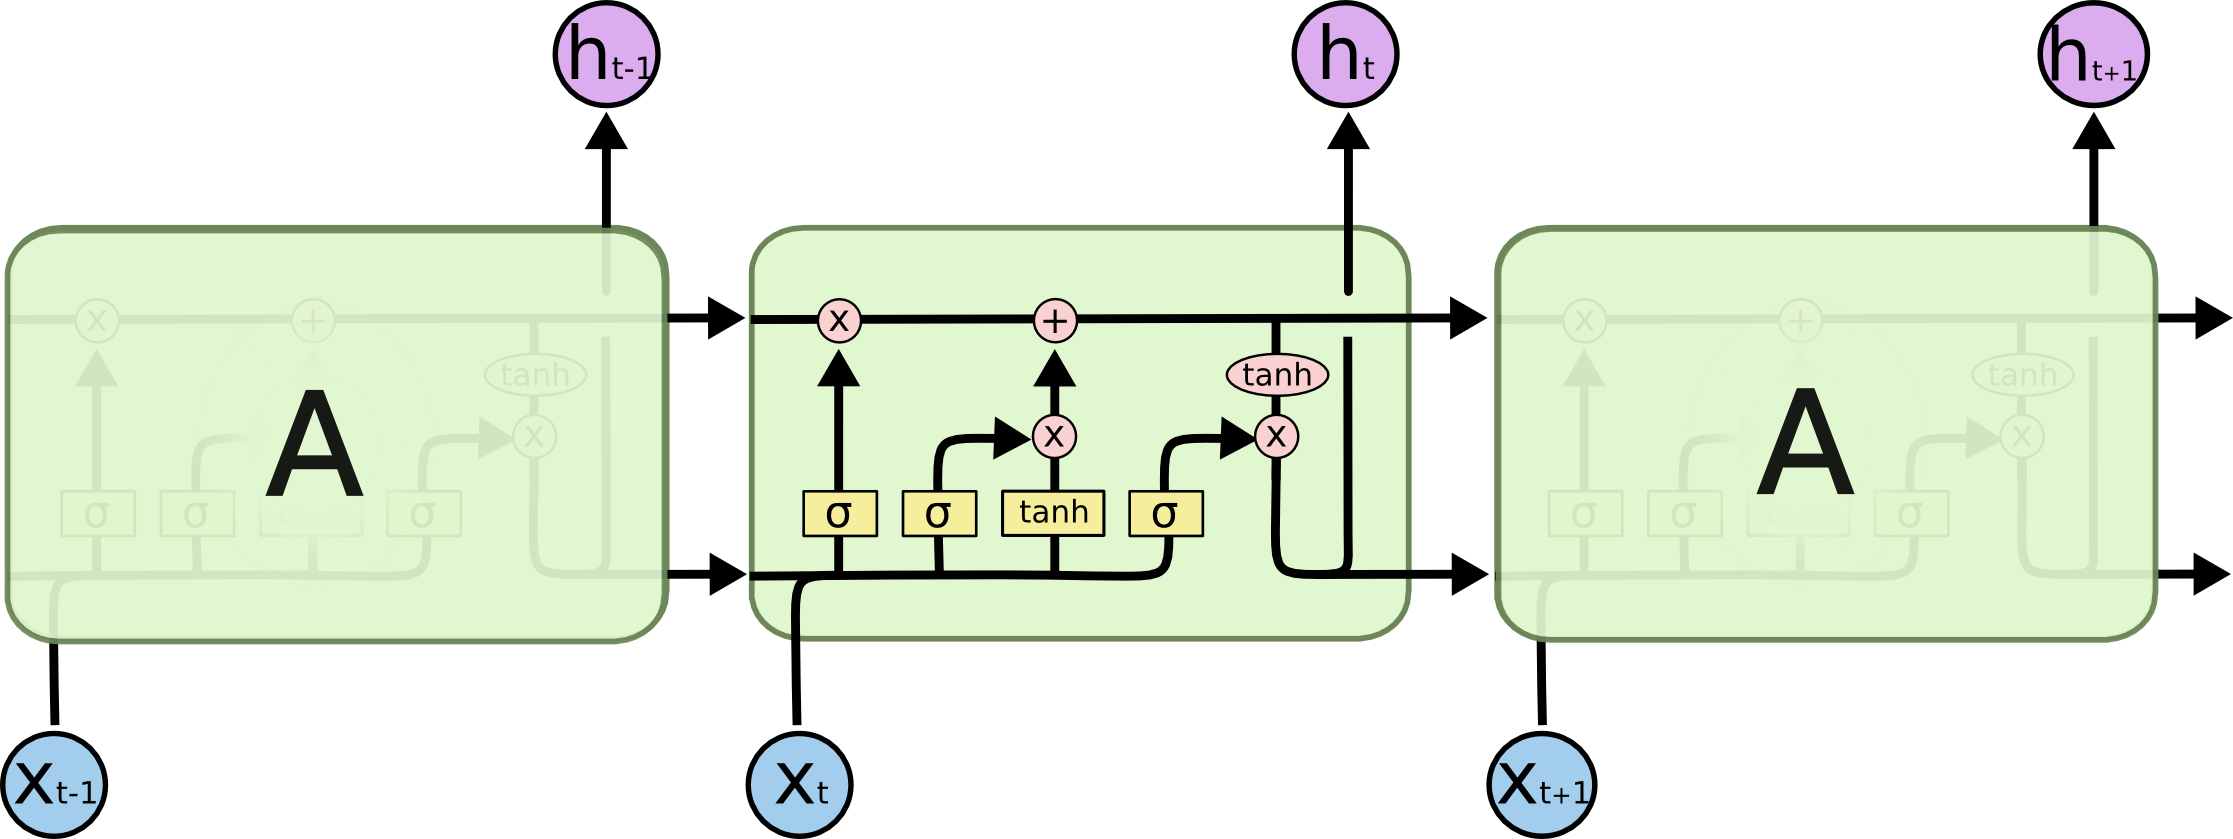
\includegraphics[scale=0.3]{LSTM3-chain.png}
\label{}
\end{figure}
\\
Полное математическое описание классического LSTM нейрона:
$$ f_t = \sigma( W_f \cdot [h_{t-1},x_t] + b_f) $$
$$ i_t = \sigma( W_i \cdot [h_{t-1},x_t] + b_i) $$
$$ \tilde{C_t} = tanh( W_C \cdot [h_{t-1},x_t] + b_C) $$
$$ C_t = f_t * C_{t-1} + i_t * \tilde{C_t} $$
$$ o_t = \sigma( W_o \cdot [h_{t-1},x_t] + b_o) $$
$$ h_t = o_t * tanh(c_t) $$
\\
\\
GRU нейрон это, по сути, упрощенная версия LSTM нейрона:
\begin{figure}[H]
\centering
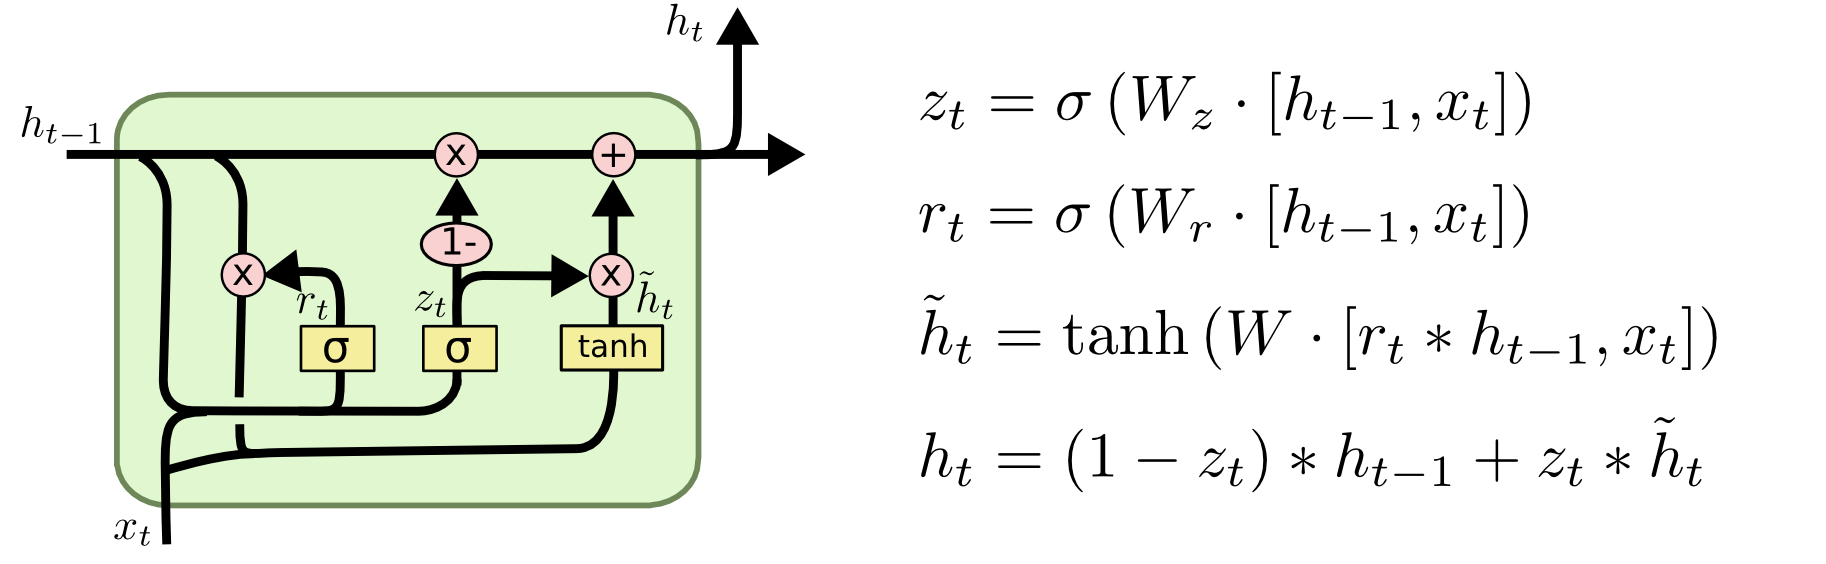
\includegraphics[scale=0.50]{LSTM3-var-GRU.png}
\label{}
\end{figure}
В данном нейроне вектор выходов $h_t$ так же "выполняет"\ роль вектора контекста, и используются следующие блоки:
\begin{itemize}
\item Блок обновления $z_t(x_t,h_{t-1};W_z)$, рассчитывающий веса в диапазоне $(0,1)$, которые применяются для рассчета нового вектора выходов (и, одновременно, контекста) $h_t$ исходя из вектора-кандидата $\tilde{h}_t$ и предыдущего вектора $h_{t-1}$
\item Блок "релевантности"\ $r_t(x_t,h_{t-1};W_r)$, рассчитывающий веса в диапазоне $(0,1)$, которые определяют "релевантность"/"важность"\ значений предыдущего выходного вектора $h_{t-1}$ при рассчете вектора-кандидата для нового выходного вектора $\tilde{h}_t$
\item Блок рассчета вектора-кандидата новых выходов $\tilde{h}_t(x_t,h_{t-1},r_t;W)$
\item Блок рассчета нового вектора выходов $h_t(h_{t-1},\tilde{h}_t,z_t)$ как взвешенной суммы соответствующих значений из предыдущего вектора $h_{t-1}$ и нового вектора-кандидата $\tilde{h}_t$, где веса для значений под индексом $i$ выбираются как $1-z_t[i]$ и $z_t[i]$ соответственно.
\end{itemize}
\textbf{Регрессионные деревья, boosting, bagging, гибридные подходы}.
\\
Регрессионные деревья — это метод регрессии, основанный на древовидном рекурсивном разбиении входного пространства на регионы [1]. Используя обучающую выборку выполняется рекурсивная настройка правил, разбивающих пространство $ \mathbb{R}^n $ на регионы, называемые конечными листьями. Получившийся набор правил можно представить в виде дерева решений, которые рекурсивно применяются к входному вектору $x$ и определяют конечный лист, к региону которого принадлежит этот вектор: $ d(x) = i, i=1,...,L$ где $L$ - количество конечных листьев дерева. Финальный прогноз для заданного вектора определяется как среднее выходное значение всех примеров из обучающей выборки, которые принадлежат соответствующему региону:
$$ f(x) = \frac{\sum_{j: d(x_j) = d(x)}{y_j}}{\sum_{j: d(x_j) = d(x)}{1}}  $$
Настройка правил/решений производится итеративно, где на каждой итерации выбирается правило, оптимизирующее определенный критерий. Наиболее известные и используемый критерии: критерий Джинни, информационный выигрыш, понижение дисперсии.
\\
При настройке и использовании единственной прогнозирующей модели часто возникают две в определенном смысле противоположных проблемы: переобучение и недостаточная точность прогноза, вызванная недостаточной сложностью выбранной модели. Эти проблемы в той либо иной степени свойственны всем вышеперечисленным методам. Для борьбы с этими проблемами часто используют подходы bagging и boosting, как по отдельности так и одновременно.
\\
Метод bagging (сокращение от bootstrap aggregatting) заключается в:
\begin{itemize}
\item генерации так называемых bootstrap тренировочных наборов вида $ D_b = \{x^{(b)}_i, y^{(b)}_i\}, b=1,...,B, i=1,...,N $ путем случайной равномерной выборки с возвратом (random sampling with replacement) из оригинального тренировочного набора $D=\{x_i, y_i\}, i=1,...N$, где $B$ - количество bootstrap выборок
\item обучении/настройки отдельной прогнозирующей модели $f_b(x)$ для каждой bootstrap выборки $D_b$
\item финальная прогнозирующая модель является усреднением выходов всех отдельных bootstrap моделей: $f(x) = \frac{1}{B}\sum_{b=1}^{B}{f_b(x)}$.
\end{itemize}
В результате применения описанной процедуры уменьшается проблема переобучения и повышается робастность финальной прогнозирующей модели, что позволяет уменьшить дисперсию ошибки прогноза как в теории [2] так и на практике [3]. Применение bagging подхода к регрессионным деревьям также известно как метод случайного леса [4], и существует множество различных модификаций ([5][6]).
\\
Метод boosting также использует несколько прогнозирующих моделей для рассчета финального прогноза, но другим образом. Существует большое количество различных boosting алгоритмов, большинство из них можно описать следующей схемой:
\begin{itemize}
\item Построение прогнозирующих моделей происходит итеративно, каждая следующая модель обучается прогнозировать разницу между суммой прогнозов уже обученных моделей и реальным значением.
\item Соответственно, самая первая модель обучается прогнозировать исходный временной ряд.
\item В некоторых вариациях, при новой итерации обучения модели также используют т.н. "перевзвешивание" примеров из обучающей выборки, когда в функции ошибки для обучения новой модели используется взвешенная сумма ошибок для отдельных примеров $L(f) = \sum_{i=1}^{N}{\theta_il(f(x_i), y_i)}$ и веса для "хороших"\ примеров с малой ошибкой на предыдущей итерации уменьшаются а веса для "плохих"\ примеров увеличиваются, таким образом "фокусируя"\ новую модель на улучшение прогноза именно для этих примеров. Вместо использования взвешенной суммы ошибок также возможно использования семплирования примеров в новую обучающую выборку, где вероятность семплирования конкретного примера обратно пропорциональна значению ошибки прогноза на предыдущей итерации.
\item Остановка итераций осуществляется при выполнении определенного критерия, после чего финальная прогнозирующая модель является взвешенной суммой прогнозов отдельных моделей:
$$ f(x) = \sum_{i=1}^{M}{w_if_i(x)}, $$
где $M$ - общее количество итераций, $ f_i(x) $ - модель, обученная на $i$-ой итерации.
\end{itemize}
Применение boosting также уменьшает дисперсию ошибки и влияние проблемы overfitting. Кроме этого, boosting позволяет использовать простые и не очень точные модели на каждой итерации (например небольшие регрессионные деревья), т.н. weak learners, для получения сложной и точной финальной модели, т.н. strong learner, таким образом адресуя проблему недостаточной сложности отдельных прогнозирующих моделей.
\\
Многие современные работы, посвященные задаче прогнозирования, фокусируются на использовании гибридов нескольких из описанных подходов:
\begin{itemize}
\item В работе [7] авторы предлагают комбинацию прогнозирующей модели ARIMA и искусственных нейронных сетей, где в нейронную сеть передаются предыдущие значения временного ряда $x_t,x_{t-1},...,x_{t-n}$, текущий прогноз ARIMA модели $\hat{L}_t$ и ошибки предыдущих прогнозов ARIMA модели $r_t,r_{t-1},...,r_{t-n};r_i=x_i-\hat{L}_i$.
\item Похожий подход предложен в [8], где для моделирования линейной составляющей временного ряда используется сезонная ARIMA модель, а для моделирования нелинейной составляющей используется метод опорной векторной регрессии с применением нелинейного ядра, модифицированного критерия оптимизации и алгоритма светлячка (firefly algorithm) для оптимизации этого критерия.
\item В работе [9] предлагается использование искусственной нейронной сети состоящие из нео-нечетких нейронов и применение МГУА-подобного алгоритма для автоматического подбора структуры и параметров сети. Нео-нечеткий нейрон является системой нечеткого вывода и реализует следующую функцию:
$$ y(x_1,x_2) = f_1(x_1) + f_2(x_2); f_i(x_i) = \sum_{j=1}^{n}{w_{ji}\mu_{ji}(x_i)},  $$
где $\mu_{ji}$ - функция принадлежности к нечеткому множеству (наиболее популярными вариантами являются гауссова ф.п., треугольная ф.п. и пр.), $w_{ji}$ - настраиваемый параметр.
\item тест
\end{itemize}
\section*{Recurrent Sigmoid Piecewise (RSP) нейрон}
В данной работе предлагается новая модель рекуррентного нейрона Recurrent Sigmoid Piecewise (RSP), в основе которой лежит Sigmoid Piecewise (SP) нейрон со следующей математической моделью:
$$ SP(x;w_+,w_-,s,k)=\frac{w_+ \cdot x}{1 + e^{-k(s \cdot x)}} + \frac{w_- \cdot x}{1 + e^{k(s \cdot x)}} $$
Используя обозначение сигмоидального нейрона:
$$\sigma(x;s)=\frac{1}{1+e^{s \cdot x}}$$
и $k=1$ получаем:
$$ SP(x;w_+,w_-,s)=\sigma(x;s)(w_+ \cdot x) + \sigma(x;-s)(w_- \cdot x) $$
Используя равенство $\sigma(x;-s)=1 - \sigma(x;s)$:
$$ SP(x;w_+,w_-,s) = (1 - \sigma(x;s))(w_- \cdot x) + \sigma(x;s)(w_+ \cdot x) $$
Если вместо одного SP нейрона описывается слой из N нейронов, то вместо векторов $w_+,w_-,s$ будут использоваться матрицы $W_+,W_-,S$:
$$ SP(x;W_+,W_-, S) = (1 - \sigma(x;S)) * (W_- \cdot x) + \sigma(x;S) * (W_+ \cdot x) $$
Введя обозначения $ z = \sigma(x;S) $, $a = W_- \cdot x$ и $b = W_+ \cdot x$ получаем:
$$ SP(x) = (1 - z) * a + z * b $$
Что очень похоже на блок рассчета нового вектора выходов в нейроне GRU:
$$ h_t = (1-z_t)*h_{t-1} + z_t*\tilde{h}_t. $$
Таким образом, слегка изменив SP нейрон, можно получить его рекуррентную версию, Recurrent Sigmoid Piecewise (RSP) нейрон, который принимает на вход вектор $p_t=[h_{t-1}, x_t]$ и выдает $h_t$:
$$ h_t=RSP(p_t;W_c,S) = (1-\sigma(p_t;S))*p_t + \sigma(p_t;S)*(W_c \cdot p_t) $$
Либо же, по аналогии с LSTM/GRU нейронами, мат. модель RSP нейрона можно записать в несколько этапов/блоков:
$$ z_t = \sigma(S \cdot [h_{t-1}, x_t]) $$
$$ \tilde{h}_t = W_c \cdot [h_{t-1}, x_t] $$
$$ h_t = (1 - z_t) * h_{t-1} + z_t * \tilde{h}_t $$
\\
И представить их в виде структурной схемы:
\\
\begin{figure}[H]
\centering
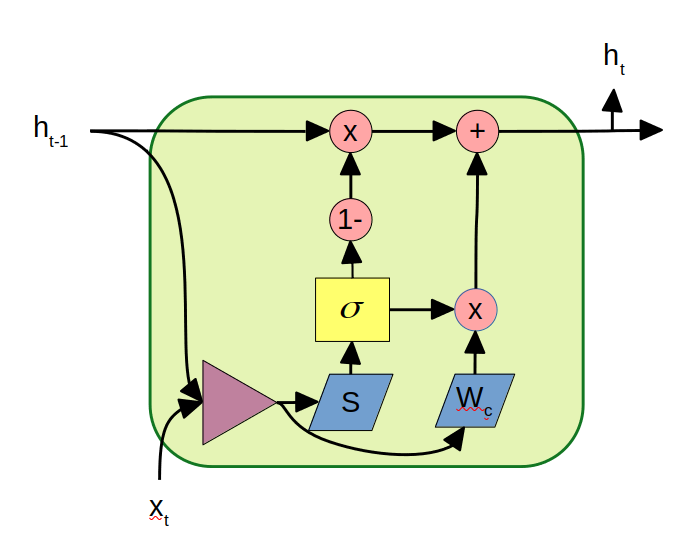
\includegraphics[scale=0.3]{recurrent_sigmoid_piecewise_neuron_structure.png}
\label{}
\end{figure}

Поверхностно сравнив RSP нейрон с LSTM и GRU нейронами можно сделать следующие наблюдения:
\begin{itemize}
\item Математическая модель RSP нейрона проще (используется лишь один нелинейный сигмоидальный блок) чем модели LSTM и GRU нейронов. В задаче прогнозирования временных рядов более простые модели часто предпочтительны на практике.
\item По сравнению с LSTM нейроном, RSP нейрон имеет в 2 раза меньше настраиваемых параметров (2 матрицы весовых коэффициентов в RSP нейроне против 4 матриц в LSTM). По сравнению с GRU нейроном - RSP имеет в 1.5 раз меньше параметров (2 матрицы вместо 3 в GRU).
\item При этом, RSP так же как и LSTM и GRU нейроны позволяет забывать определенные значения в векторе контекста при необходимости.
 
\end{itemize}
  

\section*{Практическое сравнение нейронов RSP, LSTM, GRU}
Для оценки эффективности применения RSP нейрона в моделировании прогнозируемого временного ряда были использованы два реальных временных ряда:
\begin{enumerate}
  \item Ежедневные значения индекса Доу-Джонса за период 2015/01/01-2023/1/1, общая длина временного ряда - 2014 значений [x]:
\begin{figure}[H]
\centering
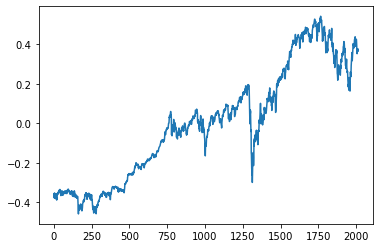
\includegraphics[scale=0.5]{dji_2015_01_01_2023_01_01.png}
\label{}
\end{figure}
  \item Временной ряд OT (oil temperature, температура масла в электрическом трансформере) из набора данных Electricity Transformer Dataset, который часто используют для оценки методов прогнозирования, общая длина временного ряда - 5000 значений [x]:
\begin{figure}[H]
\centering
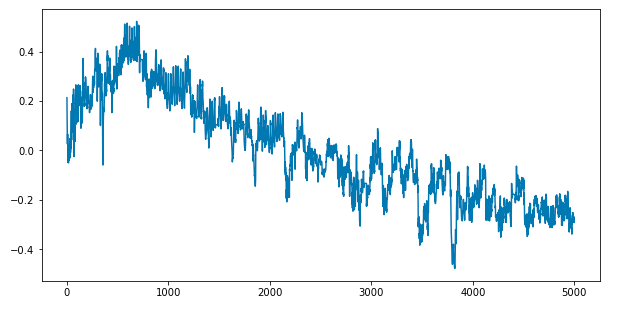
\includegraphics[scale=0.5]{etth_ot_time_series.png}
\label{}
\end{figure}
\end{enumerate}

Указанные ряды разбивались на обучающую и тестовую выборки, после чего параметры моделей настраивались на обучающей выборке и рассчитывались метрики на тестовой выборке.
Для приведения исходного временного ряда к "более стационарному виду"\ для каждой обучающей выборки сначала был подобран оптимальный линейный предиктор, после чего перед соответствующей рекуррентной сетью ставилась задача прогнозирования отклонения реального значения временного ряда от прогноза линейного предиктора.
Два предыдущих значения временного ряда использовались как вход в сеть для прогнозирования следующего значения; коэффициент обучения для всех моделей равен 0.001; максимальное количество епох обучения - 300. 
Для сравнения RSP нейрона с нейронами LSTM и GRU в различных конфигурациях сети перебирались следующие возможные значения структурных гиперпараметров: количество слоев модели $\in [1, 3, 5]$, размерность скрытого вектора состояния $\in [4, 8, 32]$.
\\
Итого, учитывая 3 выбора для типа нейрона, 3 выбора для количества слоев и 3 выбора для размерности скрытого вектора состояния для каждого из 2 временных рядов обучалось 27 различных моделей. Для каждой модели рассчитывались и запоминались значения ошибки на тестовой выборке 1 раз в каждые 20 епох обучения, также запоминалось время, затрачиваемое на выполнение каждой епохи. Резюме полученных результатов предоставлено в следующих таблицах:
\\
\begin{table}[H]
\caption{Показатели различных конфигураций моделей для временного ряда индекса Доу-Джонса}
\begin{tabular}{|p{1.4cm}|p{1.4cm}|p{1.4cm}|p{1.5cm}|p{2.5cm}|p{1.9cm}|p{2cm}|}
\hline
Количе-ство слоев &  Размер-ность вектора h & Тип нейрона & Лучшая тестовая ошибка & Относительная лучшая тестовая ошибка & Среднее время на эпоху (с) & Относитель-ное среднее время на эпоху \\
\hline
 1 &   4 &   RSP & 0.0065 & 1.0427 & 0.5714 &  1.0000 \\
\hline
 1 &   4 &   GRU & 0.0080 & 1.2818 & 0.6393 &  1.1187 \\
\hline
 1 &   4 &  LSTM & 0.0062 & 1.0000 & 0.7121 &  1.2461 \\
\hline
 1 &   8 &   RSP & 0.0063 & 1.0236 & 0.5749 &  1.0000 \\
\hline
 1 &   8 &   GRU & 0.0063 & 1.0176 & 0.6477 &  1.1266 \\
\hline
 1 &   8 &  LSTM & 0.0062 & 1.0000 & 0.7148 &  1.2434 \\
\hline
 1 &  32 &   RSP & 0.0062 & 1.0000 & 0.5790 &  1.0000 \\
\hline
 1 &  32 &   GRU & 0.0062 & 1.0001 & 0.6602 &  1.1404 \\
\hline
 1 &  32 &  LSTM & 0.0063 & 1.0128 & 0.7805 &  1.3482 \\
\hline
 3 &   4 &   RSP & 0.0068 & 1.0794 & 1.3176 &  1.0000 \\
\hline
 3 &   4 &   GRU & 0.0063 & 1.0000 & 1.5118 &  1.1475 \\
\hline
 3 &   4 &  LSTM & 0.0067 & 1.0753 & 1.8286 &  1.3879 \\
\hline
 3 &   8 &   RSP & 0.0067 & 1.0796 & 1.3112 &  1.0000 \\
\hline
 3 &   8 &   GRU & 0.0063 & 1.0292 & 1.5177 &  1.1575 \\
\hline
 3 &   8 &  LSTM & 0.0062 & 1.0000 & 1.8187 &  1.3870 \\
\hline
 3 &  32 &   RSP & 0.0062 & 1.0097 & 1.3277 &  1.0000 \\
\hline
 3 &  32 &   GRU & 0.0062 & 1.0041 & 1.5323 &  1.1541 \\
\hline
 3 &  32 &  LSTM & 0.0061 & 1.0000 & 1.9881 &  1.4975 \\
\hline
 5 &   4 &   RSP & 0.0063 & 1.0179 & 2.0749 &  1.0000 \\
\hline
 5 &   4 &   GRU & 0.0069 & 1.0998 & 2.4140 &  1.1635 \\
\hline
 5 &   4 &  LSTM & 0.0062 & 1.0000 & 2.9418 &  1.4178 \\
\hline
 5 &   8 &   RSP & 0.0065 & 1.0263 & 2.0498 &  1.0000 \\
\hline
 5 &   8 &   GRU & 0.0063 & 1.0000 & 2.4031 &  1.1724 \\
\hline
 5 &   8 &  LSTM & 0.0071 & 1.1170 & 2.9154 &  1.4223 \\
\hline
 5 &  32 &   RSP & 0.0065 & 1.0409 & 2.0939 &  1.0000 \\
\hline
 5 &  32 &   GRU & 0.0062 & 1.0067 & 2.4391 &  1.1649 \\
\hline
 5 &  32 &  LSTM & 0.0062 & 1.0000 & 3.1976 &  1.5271 \\
\hline
\end{tabular}
\end{table}

\begin{table}[H]
\caption{Показатели различных конфигураций моделей для временного ряда OT ETTH}
\begin{tabular}{|p{1.4cm}|p{1.4cm}|p{1.4cm}|p{1.5cm}|p{2.5cm}|p{1.9cm}|p{2cm}|}
\hline
Количе-ство слоев &  Размер-ность вектора h & Тип нейрона & Лучшая тестовая ошибка & Относительная лучшая тестовая ошибка & Среднее время на эпоху (с) & Относитель-ное среднее время на эпоху \\
\hline
1 &   4 &   RSP & 0.0030 & 1.0030 & 1.4462 &  1.0000 \\
\hline
1 &   4 &   GRU & 0.0030 & 1.0000 & 1.6299 &  1.1270 \\
\hline
1 &   4 &  LSTM & 0.0031 & 1.0334 & 1.8409 &  1.2729 \\
\hline
1 &   8 &   RSP & 0.0030 & 1.0000 & 1.4436 &  1.0000 \\
\hline
1 &   8 &   GRU & 0.0030 & 1.0240 & 1.6246 &  1.1254 \\
\hline
1 &   8 &  LSTM & 0.0030 & 1.0021 & 1.8294 &  1.2672 \\
\hline
1 &  32 &   RSP & 0.0029 & 1.0000 & 1.4709 &  1.0000 \\
\hline
1 &  32 &   GRU & 0.0030 & 1.0072 & 1.6553 &  1.1254 \\
\hline
1 &  32 &  LSTM & 0.0030 & 1.0164 & 1.9888 &  1.3521 \\
\hline
3 &   4 &   RSP & 0.0031 & 1.0129 & 3.3214 &  1.0000 \\
\hline
3 &   4 &   GRU & 0.0031 & 1.0000 & 3.9134 &  1.1782 \\
\hline
3 &   4 &  LSTM & 0.0032 & 1.0281 & 4.6709 &  1.4063 \\
\hline
3 &   8 &   RSP & 0.0031 & 1.0181 & 3.2960 &  1.0000 \\
\hline
3 &   8 &   GRU & 0.0030 & 1.0014 & 3.9221 &  1.1899 \\
\hline
3 &   8 &  LSTM & 0.0030 & 1.0000 & 4.6470 &  1.4099 \\
\hline
3 &  32 &   RSP & 0.0030 & 1.0225 & 3.3440 &  1.0000 \\
\hline
3 &  32 &   GRU & 0.0029 & 1.0000 & 3.9690 &  1.1869 \\
\hline
3 &  32 &  LSTM & 0.0030 & 1.0269 & 5.0812 &  1.5195 \\
\hline
5 &   4 &   RSP & 0.0030 & 1.0000 & 5.2663 &  1.0000 \\
\hline
5 &   4 &   GRU & 0.0031 & 1.0200 & 6.1705 &  1.1717 \\
\hline
5 &   4 &  LSTM & 0.0032 & 1.0841 & 7.6743 &  1.4573 \\
\hline
5 &   8 &   RSP & 0.0030 & 1.0000 & 5.2238 &  1.0000 \\
\hline
5 &   8 &   GRU & 0.0031 & 1.0413 & 6.1681 &  1.1808 \\
\hline
5 &   8 &  LSTM & 0.0031 & 1.0230 & 7.6274 &  1.4601 \\
\hline
5 &  32 &   RSP & 0.0030 & 1.0098 & 5.3234 &  1.0000 \\
\hline
5 &  32 &   GRU & 0.0030 & 1.0198 & 6.2275 &  1.1698 \\
\hline
5 &  32 &  LSTM & 0.0029 & 1.0000 & 8.3525 &  1.5690 \\
\hline
\end{tabular}
\end{table}

Где "относительная лучшая тестовая ошибка"\ и "относительное среднее время на эпоху"\ рассчитывались путем деления соответствующего абсолютного значения на минимальное значение среди всех 3 типов нейронов для данной конфигурации структурных гиперпараметров. То есть для каждой конкретную конфигурацию количества слоев и размерности скрытого вектора состояния h в предыдущих 2 таблицах есть 3 строки, по одной для каждого типа нейрона; тогда среди этих 3 строк стока для нейрона с наименьшей абсолютной лучшей тестовой ошибкой будет иметь значение относительной лучшей тестовой ошибки равное 1, а все остальные - некоторые значения >= 1, аналогично для абсолютного и относительного среднего времени на эпоху.
\\
Если усреднить относительные параметры для каждого нейрона по всем возможным конфигурациям получим следующие результаты:

\begin{table}[H]
\caption{Усредненные результаты для временного ряда индекса Доу-Джонса}
\begin{tabular}{ |p{2.2cm}|p{5cm}|p{5cm}|  }
 \hline
  Тип нейрона & Средняя относительная лучшая тестовая ошибка & Среднее относительное время на эпоху \\
  \hline
 RSP & 1.03556 & 1.0 \\
 \hline  
 GRU & 1.0488 & 1.1495 \\
 \hline 
 LSTM & 1.0228 & 1.38636 \\
 \hline
\end{tabular}
\end{table}

\begin{table}[H]
\caption{Усредненные результаты для временного ряда OT ETTH}
\begin{tabular}{ |p{2.2cm}|p{5cm}|p{5cm}|  }
 \hline
  Тип нейрона & Средняя относительная лучшая тестовая ошибка & Среднее относительное время на эпоху \\
  \hline
 RSP & 1.00736 & 1.0 \\
 \hline  
 GRU & 1.01264 & 1.16169 \\
 \hline 
 LSTM & 1.02377 & 1.4127 \\
 \hline
\end{tabular}
\end{table}

\begin{table}[H]
\caption{Усредненные результаты для обоих временных рядов}
\begin{tabular}{ |p{2.2cm}|p{5cm}|p{5cm}|  }
 \hline
  Тип нейрона & Средняя относительная лучшая тестовая ошибка & Среднее относительное время на эпоху \\
  \hline
 RSP & 1.02146 & 1.0 \\
 \hline  
 GRU & 1.030724 & 1.1556 \\
 \hline 
 LSTM & 1.02328 & 1.3995 \\
 \hline
\end{tabular}
\end{table}

Таким образом, для нейрона RSP:
\\
\-\ * для ряда DJI относительная наилучшая тестовая ошибка усредненная по всем конфигурациям занимает 2-е место после LSTM
\\
\-\ * для ряда OT ETTH - 1 место
\\
\-\ * относительное время на эпоху усредненное по всем конфигурация для обоих рядов равно 1.0, что примерно на 15.5\% быстрее, чем следущий "по скорости"\ нейрон - GRU.
\\ 
\-\ * если усреднить относительную наилучшую тестовую ошибку по всем конфигурациям и по обоим рядам - RSP занимает 1 место.
\\
Для оценочого сравнения быстродействия нейронов замеряем среднее время "рассчета"\ GRU и RSP нейронов среди 100000 запусков для разных значений размерности входного вектора и вектора скрытого состояния. LSTM нейрон, как известно из литературы, более медленный чем GRU.

\begin{table}[H]
\caption{Среднее время рассчета нейронов для разных размерностей входного и скрытого векторов (из 100000 попыток)}
\begin{tabular}{ |p{2cm}|p{2cm}|p{2cm}|p{2cm}|p{2cm}|p{2cm}|  }
 \hline
  Размерности векторов x и h & 8, 64 & 4, 12 &  4, 32 & 2, 8 & 2, 16 \\
  \hline
 GRU & 0.054 мс & 0.0487 мс & 0.0503 мс & 0.0492 мс & 0.0507 мс \\
 \hline 
 RSP & 0.0355 мс & 0.032 мс & 0.0327 мс & 0.0317 мс & 0.032 мс \\
 \hline
\end{tabular}
\end{table}

В среднем, время рассчета RSP нейрона в 1.58 раз меньше, чем время рассчета GRU нейрона.
   
\section*{Применение рекуррентных сетей на основе RSP нейронов для прогнозирования временных рядов}
Стандартную линейную ARMA модель можно обобщить следующим образом:
$$ X_t = \varepsilon_t + f(X_{t-1}, ..., X_{t-p}) + g(\varepsilon_{t-1},...,\varepsilon_{t-q}) ,$$
где $f: \mathbb{R}^p \to \mathbb{R}, g: \mathbb{R}^q \to \mathbb{R} $ - некоторые функции, в общем случае нелинейные. Наиболее общее описание нелинейной ARMA модели будет иметь вид:
$$ X_t = \varepsilon_t + f(X_{t-1}, ..., X_{t-p}, \varepsilon_{t-1}, ..., \varepsilon_{t-q}) ,$$
где $f: \mathbb{R}^{p+q} \to \mathbb{R}$ - нелинейная функция. На основе этого обобщения предлагается следующая схема прогнозирования временных рядов:
\begin{figure}[H]
\centering
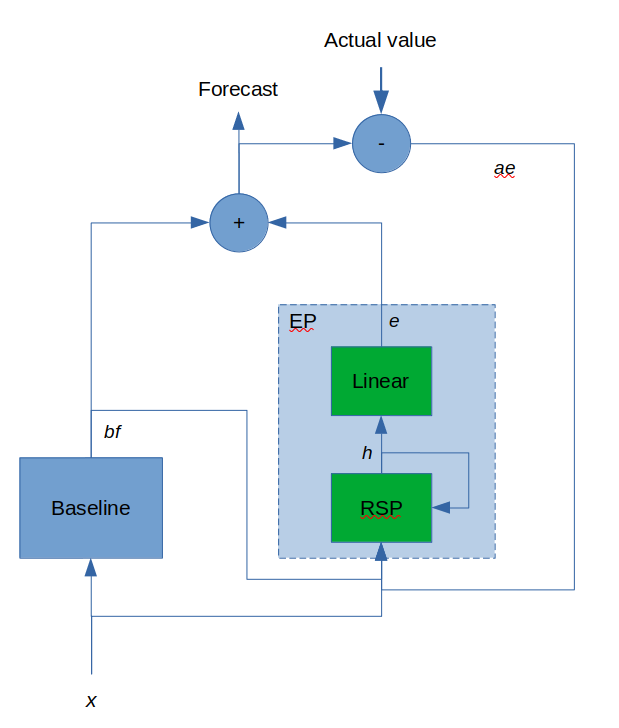
\includegraphics[scale=0.3]{rsp_forecasting_scheme.png}
\label{}
\end{figure}
где:
\begin{itemize}
\item $x$ - входной вектор, предыдущие значения часового ряда (либо нескольких рядов)
\item \textbf{Baseline} - "базисная"\ прогнозирующая модель, рассчитывающая начальную оценку прогноза, например линейная регрессия; соответственно $b_t$ - базисное значение прогноза в момент времени $t$
\item \textbf{EP} - error prediction блок, рассчитывающий оценку ошибки прогноза $\hat{e}_t$ базисного метода на основе: входного вектора, самого значения базисного прогноза и настоящей ошибки прогноза с предыдущего шага
\item Базисный прогноз $b_t$ и оценка ошибки $\hat{e}_t$ складываются для получения финального прогноза: $f_t = b_t - \hat{e}_t$
\item На следующем шаге прогнозирования $t+1$ также рассчитывается настоящая ошибка прогноза с предыдущего шага $e_{t+1} = f_{t+1} - x_{t+1}$ и передается в блок рассчета ошибки прогноза текущего шага
\item Блок рассчета ошибки состоит из RSP нейрона и простого линейного слоя. По своей математической модели RSP нейрон может "естественным" способом рассчитывать новое значение коррекции как взвешенную сумму предыдущей ошибки и нового значения контекста.
\end{itemize}

Основным отличием данной прогнозирующей схемы от обычного использования прогнозирующей модели является блок предсказания ошибки. По сути, данный блок является нелинейной вариацией MA блока в модели ARMA. Использование этого блока позволяет схеме реагировать на изменения в качестве прогноза базисной модели. Например, пускай для некоторого момента времени $t'$ получена достаточно большая ошибка прогноза $ e_{t'+1} = f_{t'+1} - x_{t'+1}, e_{t'+1} > 0 $, то есть прогноз модели оказался значительно больше реального значения. Одной из возможных причин может быть неожиданный для модели скачок "вниз" временного ряда:
\begin{figure}[H]
\centering
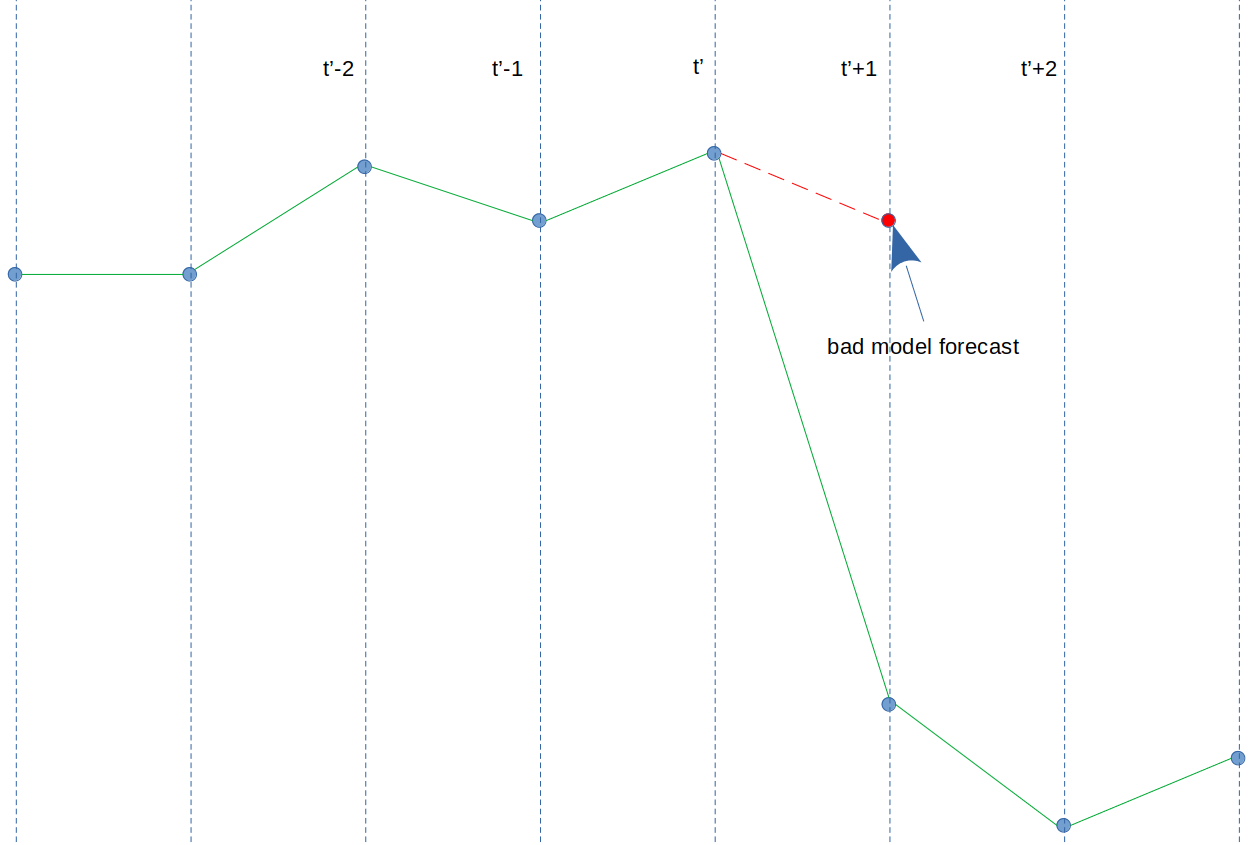
\includegraphics[scale=0.25]{bad_model_forecast_too_high_example1_for_dynamic_EC_block.png}
\label{}
\end{figure}

В таком случае можно ожидать, что в момент времени $t'+1$ прогноз базисной модели также окажется больше, и блок ПО сможет его скорректировать путем предсказания оценки ошибки $ \hat{e}_{t'+2} > 0$. И наоборот - при неожиданном скачке "вверх" на шаге $t'$ будет получена большая негативная ошибка прогноза $ e_{t'+1} < 0 $ - тогда на шаге $t'+1$ прогноз базисной модели может также быть меньше реального значения, и блок ПО сможет его скорректировать путем предсказания оценки ошибки $\hat{e}_{t'+2} < 0$.
\\ 
Преимущества данной схемы:
\begin{itemize}
\item В качестве базисной модели можно брать прогнозирующую модель, полученную в результате применения любого существующего метода прогнозирования, и таким образом в процессе обучения EP блок будет пытаться только улучшать прогноз базисной модели.
\item Рассчет настоящего значения ошибки прогноза с предыдущего шага (шагов) в теории дает возможность EP блоку динамически корректировать текущий прогноз основываясь на значениях предыдущих ошибок прогноза.
\item Мат. модель RSP нейрона естественным образом подходит для рассчета некоторой ошибки прогноза.
\item В теории возможно поэтапное обучение EP и базисного блоков - на первом этапе обучаем параметры EP блока, на втором - фиксируем их и обучаем параметры базисного блока и т.д.
\end{itemize}

\section*{Практические примеры использования подхода с блоком коррекции на основе рекуррентной RSP сети}
Для первого тестирования используем показатели сердечного ритма 4 разных пациентов в разных состояниях. В качестве базисных моделей выберем простую линейную регрессию и ансамбль регрессионных деревьев, настраиваемый с помощью градиентного бустинга, используя пакет XGBoost. Построив соответствующие базисные модели получаем следующие значения метрик качества прогноза на обучающей и тестовой выборке (усредненные по всем 4 пациентам):

\begin{tabular}{ |p{3cm}|p{3cm}|p{3cm}|p{3cm}|  }
 \hline
 Метод & MSE &  MAE & MAPE \\
 \hline
 Линейная регрессия &
 \makecell{train=0.000473 \\ test=0.00048} &
 \makecell{train=0.01283 \\ test=0.01228} &
 \makecell{train=0.058 \\ test=0.05} \\
 \hline
 XGBoost &
 \makecell{train=0.00022 \\ test=0.000479} &
 \makecell{train=0.00728 \\ test=0.0128} &
 \makecell{train=0.03818 \\ test=0.0506} \\
 \hline
\end{tabular}

Пример прогнозов линейного предиктора для одного пациента на обучающей:
\begin{figure}[H]
\centering
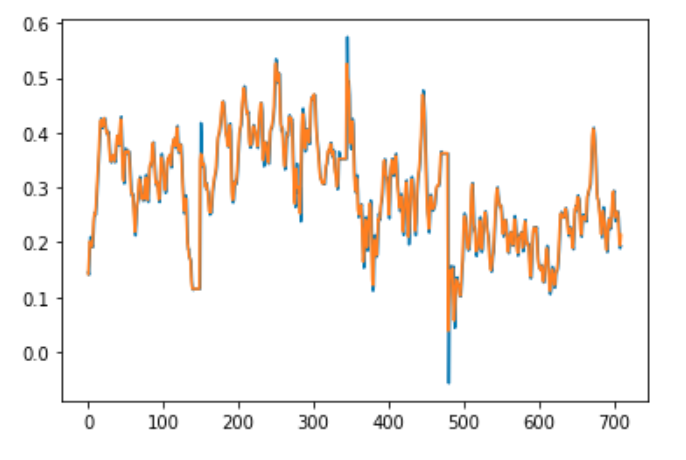
\includegraphics[scale=0.35]{baseline_train_forecast.png}
\label{}
\end{figure}
 и тестовой:
\begin{figure}[H]
\centering
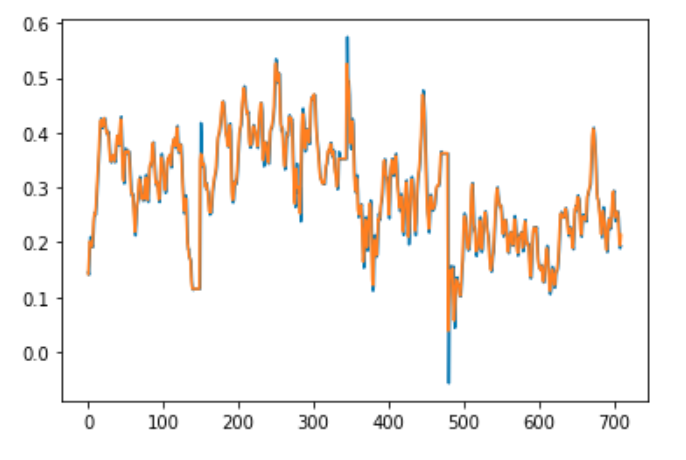
\includegraphics[scale=0.35]{baseline_train_forecast.png}
\label{}
\end{figure}
выборках.

После "фиксации"\ базисных предикторов, добавления блока корекции на основе RSP нейрона и обучения его параметров получаем следующие значения метрик:

\begin{tabular}{ |p{3cm}|p{3cm}|p{3cm}|p{3cm}|  }
 \hline
 Метод & MSE &  MAE & MAPE \\
 \hline
 Линейная регрессия с блоком коррекции &
 \makecell{train=0.00041 \\ test=0.000411} &
 \makecell{train=0.01178 \\ test=0.01145} &
 \makecell{train=0.0565 \\ test=0.047} \\
 \hline
 XGBoost с блоком коррекции &
 \makecell{train=0.000213 \\ test=0.000464} &
 \makecell{train=0.00716 \\ test=0.0125} &
 \makecell{train=0.038 \\ test=0.0502} \\
 \hline
\end{tabular}
\\
\\
где значения всех метрик для обоих методов улучшились.

В качестве второго примера возьмем временной ряд дневных значений индекса DJI за период 2015/1/1 - 2023/1/1:
\begin{figure}[H]
\centering
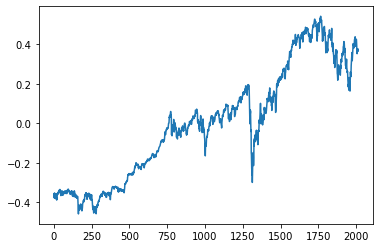
\includegraphics[scale=0.5]{dji_2015_01_01_2023_01_01.png}
\label{}
\end{figure}

Разбив данный временной ряд на обучающую и тестовую выборки:
\begin{figure}[H]
\centering
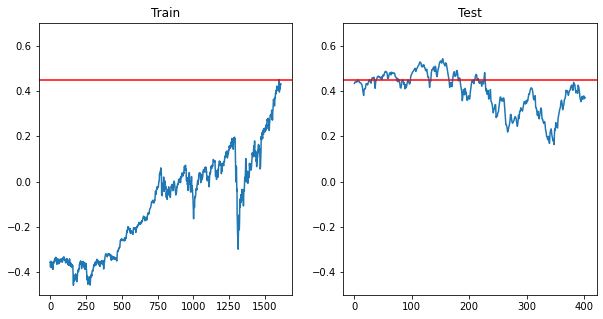
\includegraphics[scale=0.5]{dji_train_test.png}
\label{}
\end{figure}

можно заметить, что в тестовой выборке встречаются периоды, в которых значение временного ряда превышает максимальное значение, присутствующее в обучающей выборке. После настройки параметров базисных предикторов - линейной регрессии и ансамбля регрессионных деревьев - на обучающей выборке получаем следующие результаты прогнозов на тестовой выборке:
\begin{figure}[H]
\centering
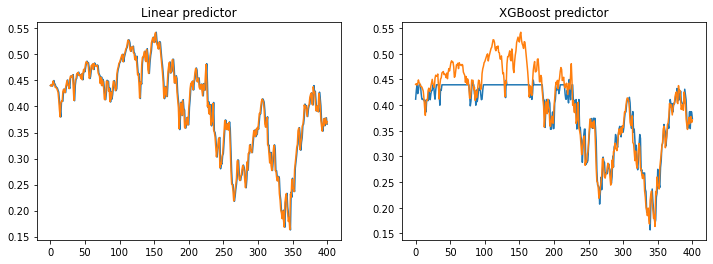
\includegraphics[scale=0.5]{/home/ivan/my_projects/nau_forecasting/docs/dji_linear_and_xgboost_test_predictions.png}
\label{}
\end{figure}
Очевидно, что ансамбль регрессионных деревьев очень плохо справился с прогнозированием значений временного ряда в соответствующих периодах. Причиной таких прогнозов является принцип построения таких деревьев, где значение прогноза для определенного входного вектора $x$ является усредненное значение выходного значения для всех примеров в листе дерева, куда попадает вектор $x$. Существуют различные методы исправления данного недостатка, однако такой случай можно рассматривать как конкретный пример проблемы непостоянного характера прогнозируемого временного ряда. Механизм коррекции, предлагаемый в данной статье, в теории способен "реагировать"\ на ухудшение качества прогноза базисного предиктора в таких ситуациях и корректировать его по возможности. Для этого, при настройке параметров блока коррекции также можно добавлять шум в прогнозы базисного предиктора, чтобы "учить"\ блок реагировать необходимым образом. Применяя этот подход получаем такой прогноз базисного предиктора XGBoost с обученным блоком коррекции на тестовой выборке:
\begin{figure}[H]
\centering
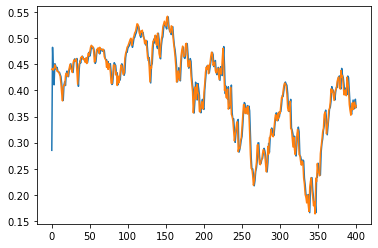
\includegraphics[scale=0.5]{dji_test_xgboost_plus_correction.png}
\label{}
\end{figure}
где хорошо видно, что добавление блока коррекции позволило существенно улучшить качество прогноза в проблемных регионах. Построив график прогнозов отдельно блока коррекции можно увидеть, как он реагирует на плохой прогноз базисного предиктора и "исправляет"\ его:
\begin{figure}[H]
\centering
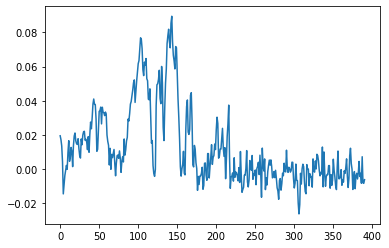
\includegraphics[scale=0.5]{dji_test_xgboost_with_correction_correction_outputs.png}
\label{}
\end{figure}

Значения метрик для базисных предикторов и вариантов с коррекцией:

\begin{tabular}{ |p{3cm}|p{3cm}|p{3cm}|p{3cm}|  }
 \hline
 Метод & MSE &  MAE & MAPE \\
  \hline
 Линейная регрессия &
 \makecell{train=0.000128 \\ test=0.0002515} &
 \makecell{train=0.0073 \\ test=0.012} &
 \makecell{train=0.1654 \\ test=0.0336} \\
 \hline
 XGBoost &
 \makecell{train=2.03*$10^{-5}$ \\ test=0.001} &
 \makecell{train=0.00328 \\ test=0.02476} &
 \makecell{train=0.09 \\ test=0.06} \\
 
 \hline
 Линейная регрессия с блоком коррекции &
 \makecell{train=0.0001276 \\ test=0.0002514} &
 \makecell{train=0.00725 \\ test=0.012} &
 \makecell{train=0.165 \\ test=0.0336} \\
 \hline
 XGBoost с блоком коррекции &
 \makecell{train=0.00011 \\ test=0.0003} &
 \makecell{train=0.00686 \\ test=0.0127} &
 \makecell{train=0.155 \\ test=0.035} \\
 \hline
\end{tabular}

\section*{Выводы и дальнейшие направления работы}

\section*{Ссылки}

\begin{enumerate}
\item Breiman L. Classification and Regression Trees. Boca Raton, FL: Chapman \& Hall; 1993.
\item BÜHLMANN, P., YU, B. Analyzing bagging. In: Annals of Statistics 30 (4), 2002, pp. 927–961.
\item BREIMAN, L. Bagging predictors. In: Machine Learning, 24(2), 1996, pp. 123–140.
\item BREIMAN, L. Random forest. In: Machine Learning 45 (1), 2001, pp. 5–32.
\item HASTIE, T., TIBSHIRANI, R., FRIEDMAN, J. The Elements of Statistical Learning. 2nd ed. New York: Springer, 2009.
\item JAMES, G., WITTEN, D., HASTIE, T., TIBSHIRANI, R. An introduction to statistical learning. In Springer 112, 2013, pp. 18.
\item Fawzy, Haitham, EL Houssainy A. Rady, and Amal Mohamed Abdel Fattah. "A Comparative Simulation Study of ARIMA and Computational Intelligent Techniques for Forecasting Time Series Data."\ Journal of Statistics Applications \& Probability Letters 11, no. 1 (2022): 1-7.
\item Ngo, Ngoc-Tri, Anh-Duc Pham, Thi Thu Ha Truong, Ngoc-Son Truong, and Nhat-To Huynh. "Developing a hybrid time-series artificial intelligence model to forecast energy use in buildings." Scientific Reports 12, no. 1 (2022): 15775.
\item Zaychenko, Yuriy, Helen Zaichenko, and Oleksii Kuzmenko. "Investigation of Artificial Intelligence Methods in the Short-Term and Middle-Term Forecasting in Financial Sphere." In System Analysis and Artificial Intelligence, pp. 307-322. Cham: Springer Nature Switzerland, 2023.

\end{enumerate}

\section*{ДИНАМИЧЕСКИЙ ВЕС, КОТОРЫЙ ПРИМЕНЯЕТСЯ К ВЫХОДУ БЛОКУ КОРРЕКЦИИ - ЧЕМ МЕНЬШЕ ПРЕДЫДУЩАЯ ОШИБКА, ТЕМ МЕНЬШЕ НЕОБХОДИМОСТЬ В КОРРЕКЦИИ НОВОГО ПРОГНОЗА И НАОБОРОТ}

\end{document}

